\chapter{The v1 synthetic generator}
\label{chap:v1gen}

This chapter documents the first iteration of the synthetic data
generator. It is kept deliberately compact because the v1 generator is
no longer the recommended pipeline; its main role in the rest of the
report is as a baseline that the v2 generator (\cref{chap:v2gen})
improves upon. The reader interested in the final pipeline can skim
this chapter and jump straight to \cref{chap:reanalysis,chap:v2gen}.

\section{Anomaly templates (v1)}
\label{sec:v1-templates}

The six v1 anomaly templates are stored as small CSV files in
\texttt{pole-anomaly-old/data-gen/anomalies/}. Each row defines a
\emph{keypoint} with six fields plus an interpolation flag; the schema
is documented in \cref{app:csv-format}. Visually, the templates fall
into four families (\cref{fig:v1-templates}):
\begin{itemize}[leftmargin=*, itemsep=0.2em]
    \item \textbf{Smooth bumps} (\texttt{bell}, \texttt{bell\_sq}):
    plumes that build up and decay smoothly, possibly with a small
    sustained plateau.
    \item \textbf{Asymmetric ramps} (\texttt{fast\_ascend},
    \texttt{fast\_descend}): rapid onset followed by slow exponential
    decay, or its time-reverse.
    \item \textbf{Plateau} (\texttt{square}): a sustained
    contamination episode.
    \item \textbf{Multi-peak} (\texttt{M}): two consecutive events with
    a dip in between.
\end{itemize}

\begin{figure}[H]
    \centering
    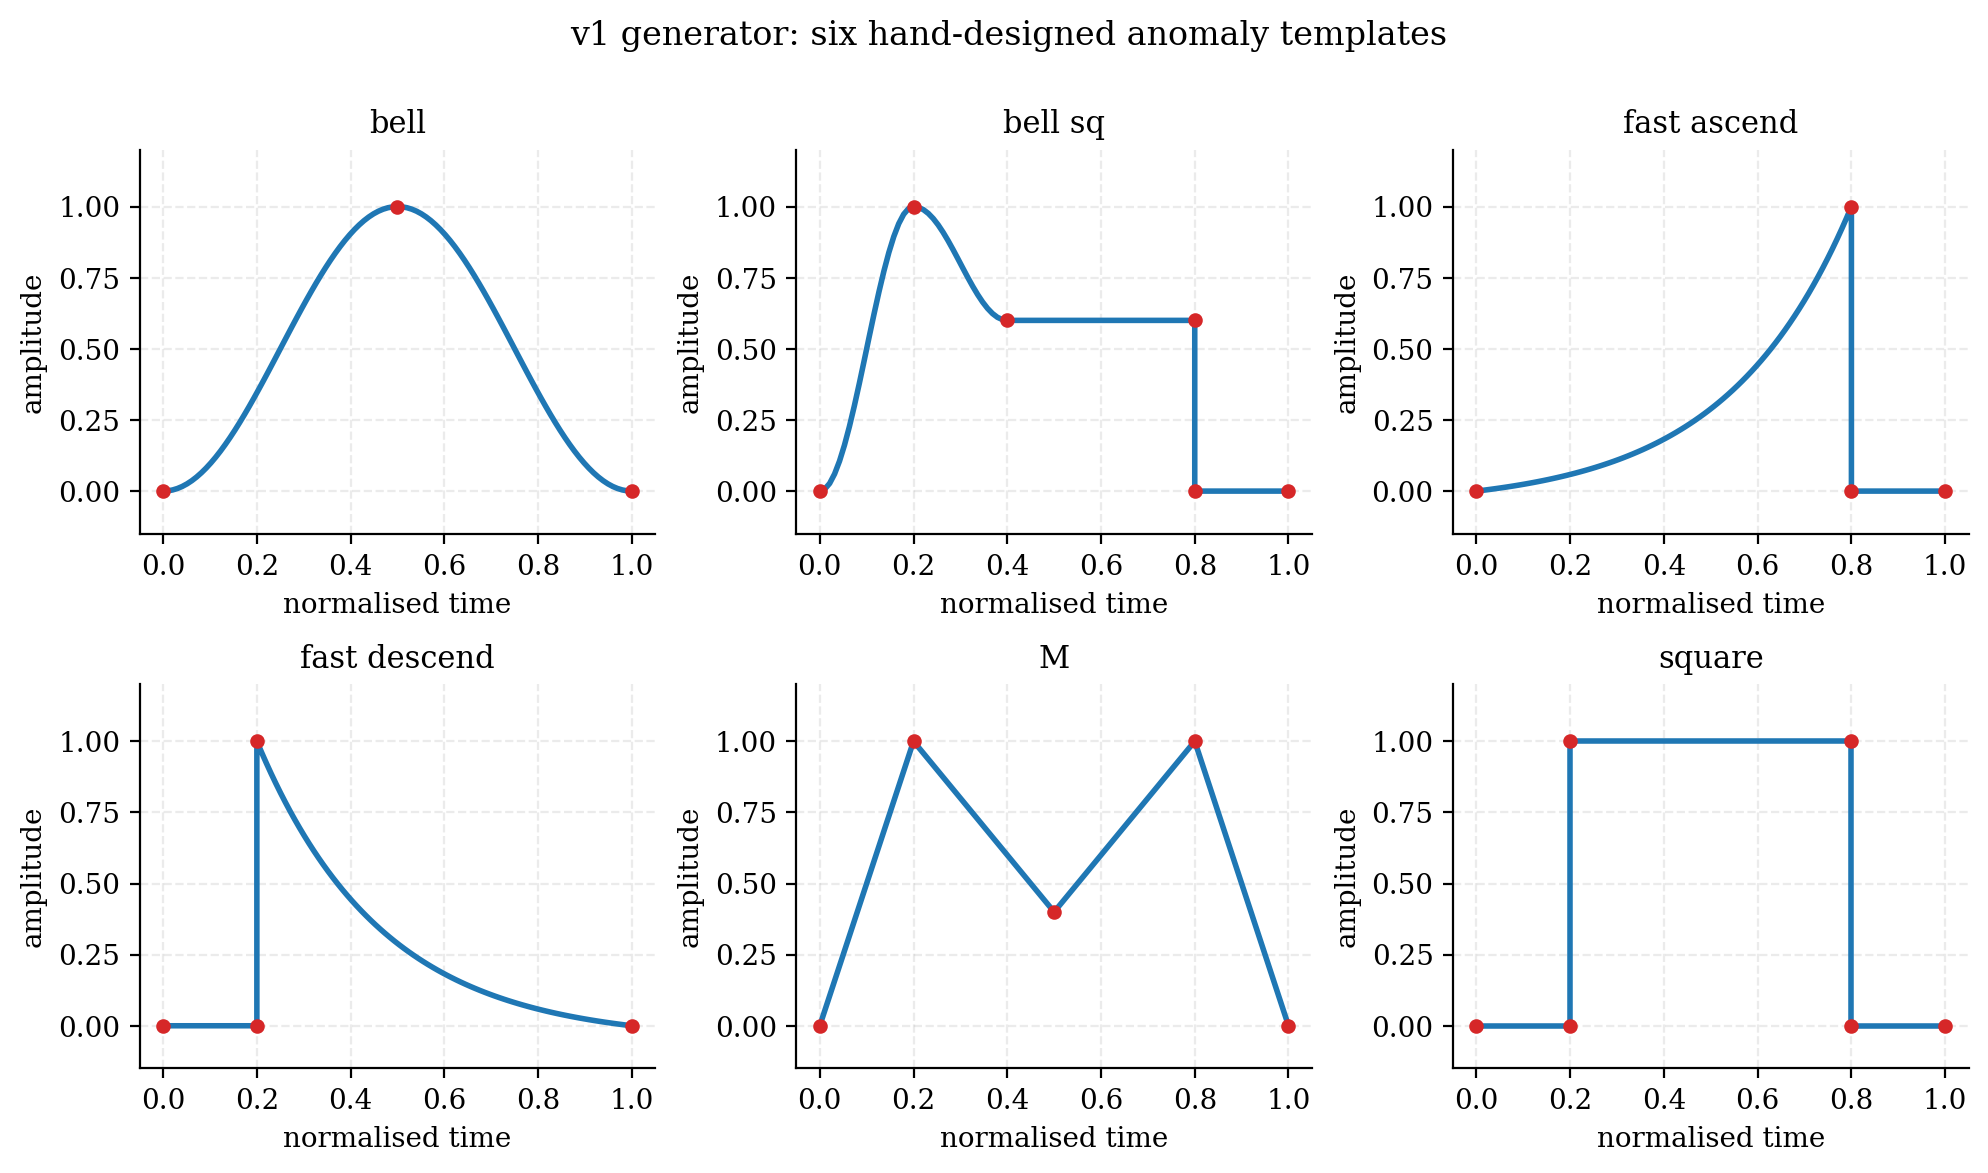
\includegraphics[width=0.95\linewidth]{figures/v1_anomaly_templates}
    \caption{The six v1 anomaly templates, drawn in normalised time and
    amplitude. Each template is encoded as a small list of keypoints
    (red dots) connected by linear, exponential or half-cosine
    (``bell'') segments.}
    \label{fig:v1-templates}
\end{figure}

\subsection{Stochastic deformation of a template}
\label{sec:v1-deformation}

A template used verbatim would not generalise. The generator therefore
\emph{deforms} each template before injecting it: each keypoint is
perturbed by an isotropic Gaussian jitter of standard deviation $\nu$
(the \emph{variance level}), then the direction constraints encoded by
the \texttt{t\_minus}, \dots, \texttt{v\_plus} flags are enforced so
that the deformed template still has the right qualitative shape (a
peak cannot become a valley, time monotonicity is enforced as a
fail-safe). The deformed keypoints are then interpolated back into a
dense curve and re-scaled to the target amplitude and period; v1 uses
\begin{equation}
    \text{amplitude} \in \sigma \cdot [\,2.5,\, 7.6\,],
    \qquad
    \text{period} \in [200,\, 800] \text{ samples},
    \qquad
    \nu \in [0.02,\, 0.10].
    \label{eq:v1-ranges}
\end{equation}
The amplitude is expressed in multiples of the high-frequency noise
standard deviation $\sigma$ from \cref{tab:real-stats}, so the
per-sample SNR of a generated anomaly lies in the interesting range
$[2.5, 7.6]$.

\begin{figure}[H]
    \centering
    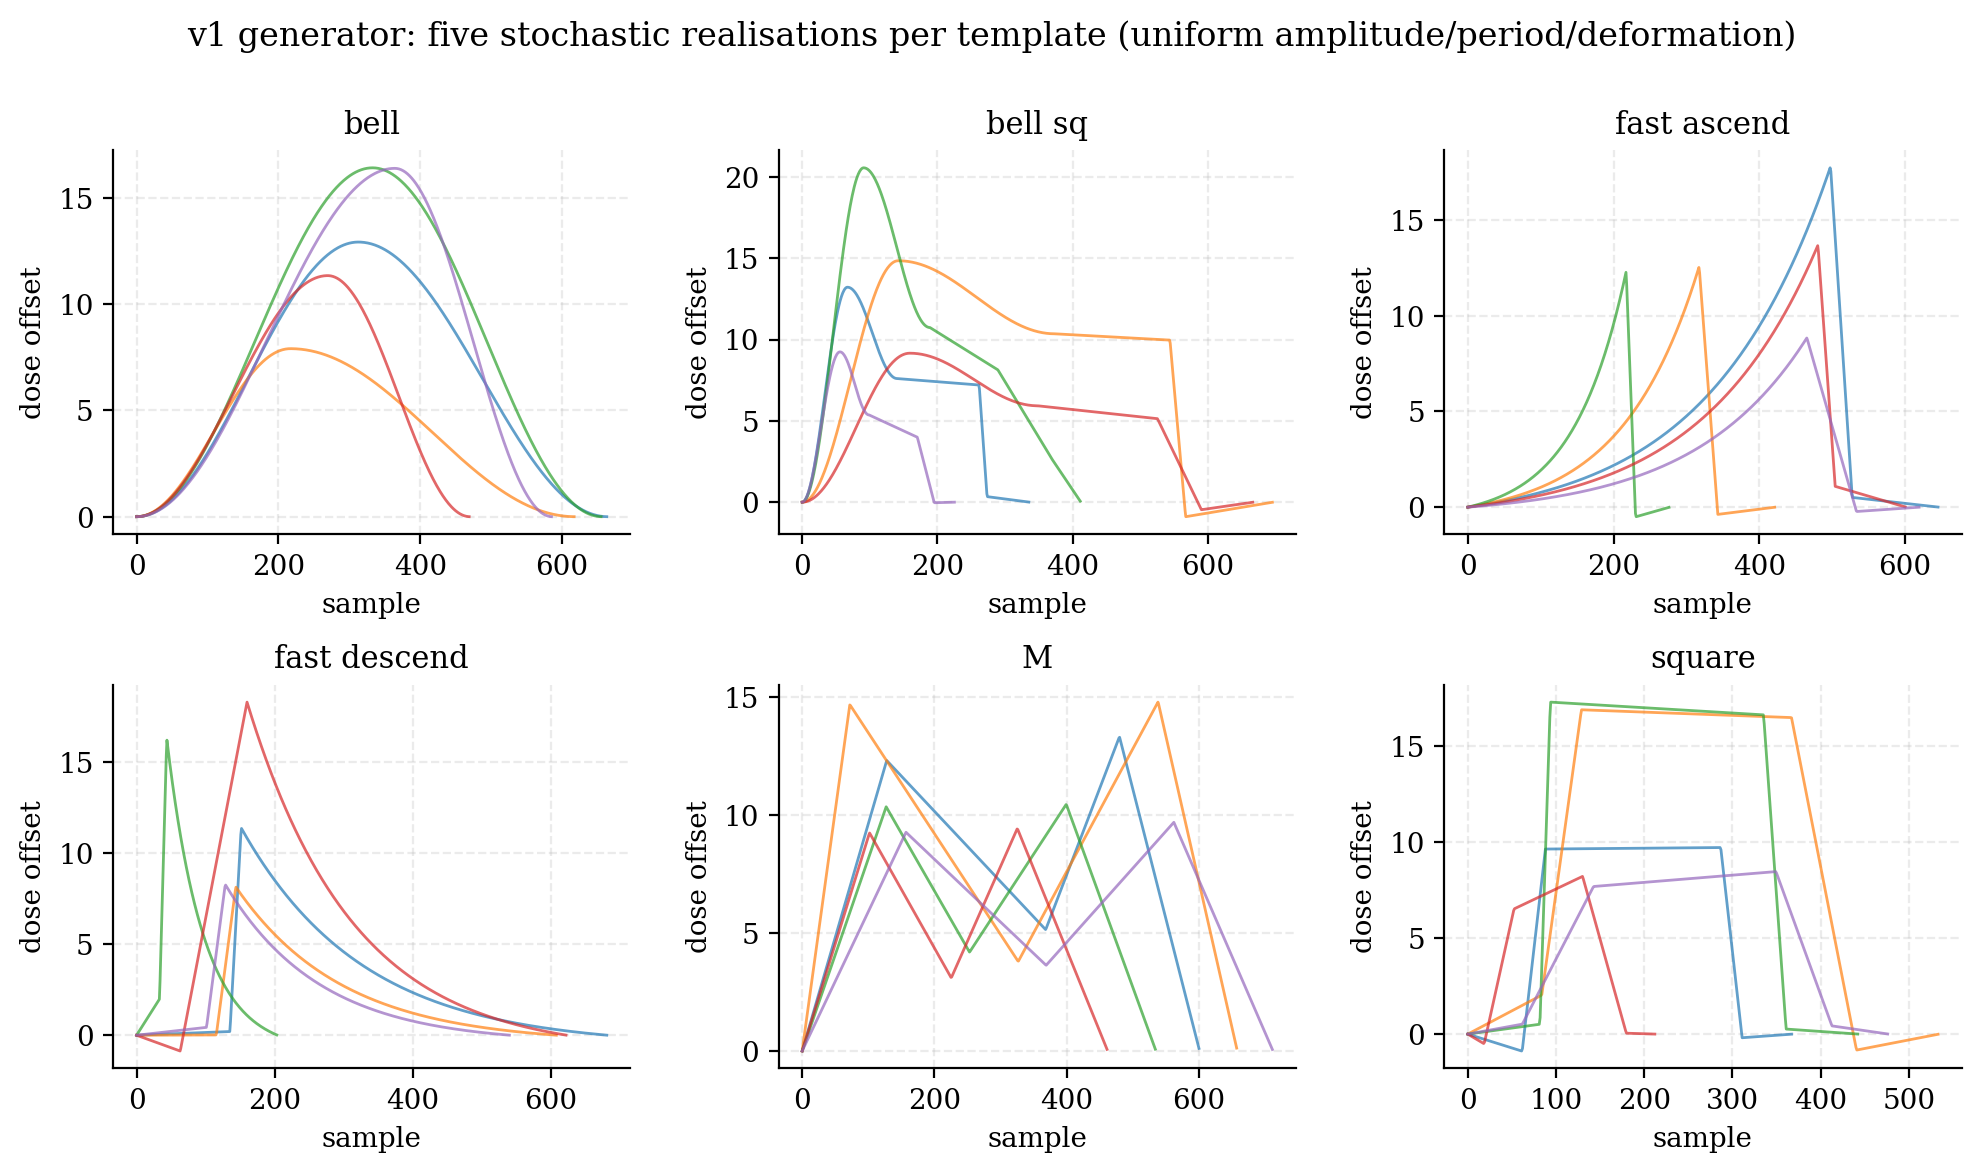
\includegraphics[width=0.95\linewidth]{figures/v1_template_deformation}
    \caption{Five stochastic realisations of each v1 template with the
    parameter ranges of \cref{eq:v1-ranges}. The qualitative shape is
    preserved, but no two realisations are identical.}
    \label{fig:v1-deformation}
\end{figure}

\section{The v1 generator algorithm}
\label{sec:v1-gen-algo}

The end-to-end generator (\texttt{generate\_custom\_dataset.py} in
\texttt{pole-anomaly-old/data-gen/}) combines the noise model of
\cref{sec:v1-noise-model} and the deformed templates of
\cref{sec:v1-deformation} into a long labelled signal. In pseudo-code,
generating $N$ points proceeds as:

\begin{enumerate}[leftmargin=*, itemsep=0.2em]
    \item Pick the total number of anomalies $M \in [5\,000, 8\,000]$
    and pre-compute their evenly-spaced injection indices, with a small
    random jitter ($\pm 200$ samples) around each grid point.
    \item For each injection point, sample a template uniformly at
    random and a triple $(\text{amplitude}, \text{period}, \nu)$ from
    the ranges of \cref{eq:v1-ranges}; produce the deformed dense
    curve.
    \item Generate the background in $50\,000$-point chunks: simulate
    the OU baseline path and overlay $\mathcal{N}(b_t, \sigma^2)$
    noise.
    \item Add each anomaly curve on top of the background at its
    injection index and label every output point with the anomaly's
    class (or $0$ if the per-point contribution falls below the
    threshold).
\end{enumerate}

The final dataset is written to disk in CSV chunks; it never lives
entirely in RAM, which lets us produce datasets of arbitrary size
within a constant memory budget.

\section{The v1 dataset used in this report}
\label{sec:v1-final-dataset}

For the v1 results in \cref{chap:v1results,chap:v1real} we generate
$N = 10^{7}$ samples and inject in the range $[5\,000, 8\,000]$
anomalies, leading to a global anomaly density of $\sim 7$ events per
$10\,000$ samples. The signal looks as in \cref{fig:v1-synth-preview}.

\begin{figure}[H]
    \centering
    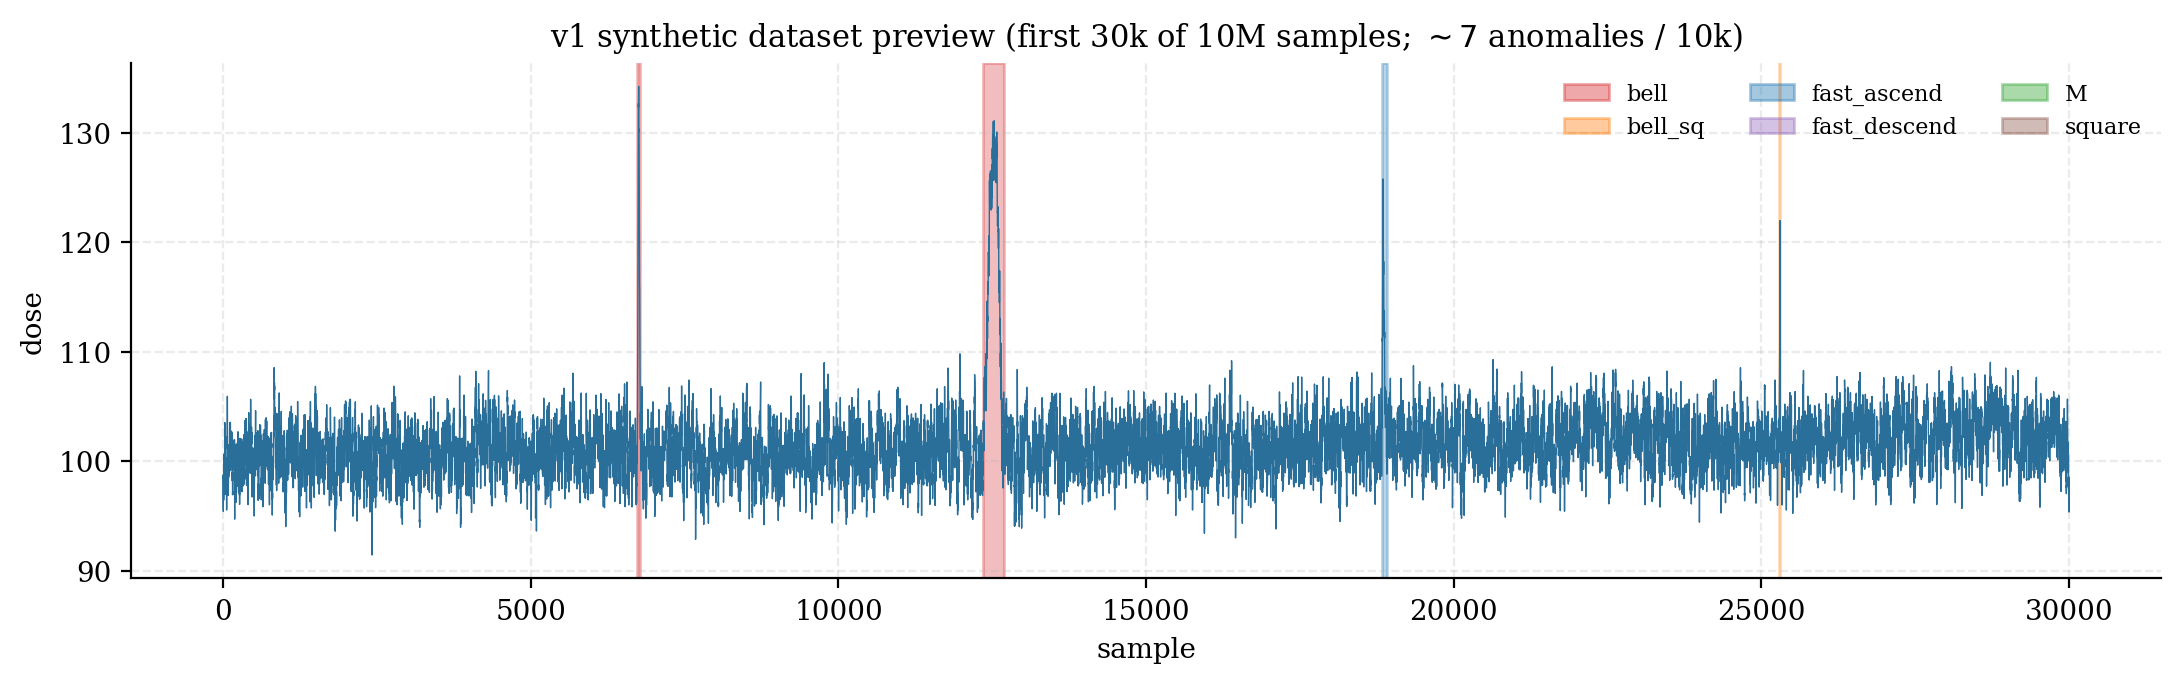
\includegraphics[width=\linewidth]{figures/v1_synthetic_preview}
    \caption{First $30\,000$ samples (of $10^{7}$) of the v1 synthetic
    dataset. Anomaly spans are coloured by class. Note the dense
    injection: roughly four visible bumps in a $30$k-sample slice.}
    \label{fig:v1-synth-preview}
\end{figure}

\section{Two v1 design choices that will matter later}
\label{sec:v1-design}

Two v1 choices, harmless on the synthetic test set, turn out to be the
main causes of the failure on real data
(\cref{chap:v1real}):

\paragraph{Dense injection.} The synthetic dataset contains roughly
one anomaly every $1\,500$ samples, whereas the real recordings contain
$17$ plausible anomalies over $4 \times 40\,000$ samples
(\cref{sec:reanalysis-labels}). The two distributions are off by a
factor of $\sim 70$ in event density --- and so the v1 training prior
of \texttt{Normal Background} is wildly off the deployment prior.

\paragraph{Templates assume clean, isolated, well-defined shapes.} The
v1 generator produces anomalies that are isolated and have a duration
in $[200, 800]$ samples. Real-life events may be much shorter (a few
samples) or much longer (multi-hour contamination), and the recordings
contain rapid, isolated single-point excursions that the templates do
not represent at all.

The next two chapters first describe the three architectures shared by
v1 and v2 (\cref{chap:archi}), then report the v1 training and
event-level evaluation on the synthetic test set (\cref{chap:v1results})
and the v1 real-data inference (\cref{chap:v1real}). Readers
familiar with the v1 results can skim them; the takeaway is that v1
works very well on synthetic data and very badly on real data.
